%*****************************************
\chapter{In-situ hybridization dataset presentation and preprocessing}\label{ch:singlecell}
%*****************************************
\section{Building a image library of gene expression in \platy{}'s brain}
     During his PhD, Raju Tomer and other members of the Arendt lab in EMBL, used wholemount in-situ hybridization to create an image library of gene expression in the brain of \platy{}. They were able to record gene expression in the full brain at 48hpf for 169 genes. In practice, each individual larvae was dissected to isolate the region containing the developing brain. Each brain was then stained with two different fluorescent probes corresponding to two messenger RNAs (mRNA). One of the genes is considered a reference, as it is always hybridized in all the assays (the main reference gene used was \emph{Emx}) alongside another gene of interest, see Figure \ref{fig:insitu}. Each brain was then visualized with laser confocal microscopy to reveal the gene expression patterns in the brain slice by slice, generating at the same time 3D coordinates for each slice.\\
     
     As mentioned previously, the larval development of \platy{} is highly similar in every individual larvae. In the case of this study where WiSH was performed on many independent animals, the stereotypical development of \platy{} has proven essential. Indeed, having the same reference gene localized in all assays allowed Tomer \emph{et al.} to align all other gene expression patterns onto this scaffold. The result is an image library of 169 gene expression patters in the full brain of \platy{} with a exploitable spatial reference that allows for a very precise mapping.\\
    
    \begin{figure}[bth]
\centerline{\includegraphics[width=1.3\linewidth]{gfx/chapter1/insitu.png}}
\caption{Wholemount in-situ hybridization ssays used to create a 169 genes catalogue of gene expression in the brain of \platy{}. From the live tissue cut into thin fixed layers, every slice is stained with a reference gene and a gene of interest that will reveal areas of expression under fluorescent microscopy. The process repeated 169 times for key genes in \platy{} neural development has been generated by \citep{Tomer10}}\label{fig:insitu}
	\end{figure}
	

\section{Spatially referenced single cell-like in-situ hybridization data}\label{sec:single_cell_insitu}
  \subsection{Dividing images into ''cells''}
  Because in-situ hybridization preserves spatial information in the tissue under study, measuring gene expression at single cell resolution from an image obtained through confocal microscopy is a matter of microscope performance and cell size. For big enough cells, single cell resolution has been documented as far back as 1989 \citep{tautz89,poulsen93}.\\
  
  When considering the \platy{} brain dataset, with current microscope technology, achieving single cell level resolution on one particular image is feasible. However, the main limitation is analysing the quantity of data involved; indeed, each brain is separated into 20 slices, for 169 genes this yields 3380 images that require inspection. This technical bottleneck can be overcome with an automated way of analysing the fluorescence images. However this is not an easy task, as the computer program required needs to be able to \emph{see} and divide the global picture into cells. Considering that all cells do not exhibit the same shape and size, constructing this \emph{cell model} is a very complicated task.\\
  
  It is for instance possible to highlight the limits of the cells and to automatically acquire those boundaries through computer vision methods. This process relies on targeting proteins in the membrane or in the extracellular matrix of the cells with specific fluorescent probes. Once the boundaries are acquired, defining every cell is a matter of finding enclosed spaces. To that end, numerous contour detection algorithms exist \citep{li95,fan01,arbelaez11}.\\
  
  Unfortunately, a dataset with the cell limits highlighted does not yet exist for \platy{}'s brain, making a precise division of the images into cells very difficult. Instead, Tomer used a simple approach that divides the images into ``cubes'' \citep{Tomer10}.


  \subsection{A simple cell model, the ''cube'' data}
  
  Every slice of \platy{}'s brain being aligned onto the reference gene scaffold (see section \ref{sec:gene_expression_lab}) for all 169 genes, the ``cube'' model simply consists of dividing each image into squares approximately the size of an average cell. In the \platy{} dataset, the size chosen was 3 \microm{2} \citep{Fischer10}. Importantly, this is actually smaller than the average cell size in \platy{}'s brain. Each slice of the brain being approximately 3 \microm{} thick, the resulting dataset, spatially referenced in 3D, will contain 3 \microm{3} cubes, each of which is associated with the luminescence data for each of the 169 genes.\\
  
  Of course this cell model is far from perfect: it assumes that every cell in the brain is roughly the same size and cubical, which is clearly not the case. Consequently, the ``cube'' model will introduce errors in the dataset. The first type of error occurs within areas where the genes under study are highly expressed. In that case, the light emission might contaminate the surrounding cubes that do not necessarily express the same gene (see Figure \ref{fig:cubeserrors}A). The second type of error is introduced by the choice of 3 \microm{3} cubes. As they are smaller than the average cell, some cubes will fall on areas that may be artificially empty. Indeed, transcription in the cells mainly happens in the nucleus. mRNA molecules then travel to the cytoplasm to be translated but they are not evenly distributed across the cell; in particular for some large cells, parts of the cytoplasm may record no expression in a cell that actually contains a lot of transcripts (see Figure \ref{fig:cubeserrors}B).\\
  
  Hence, the data will tend to exhibit spatial discontinuity and inconsistency. With this fact in mind, any automated way of interpreting this data (in the case of this thesis: clustering ``cubes'' into cell types) will have to take into account this spatial discontinuity and try as much as possible to smooth over those potential expression gaps.\\
  
    \begin{figure}[h]
\centerline{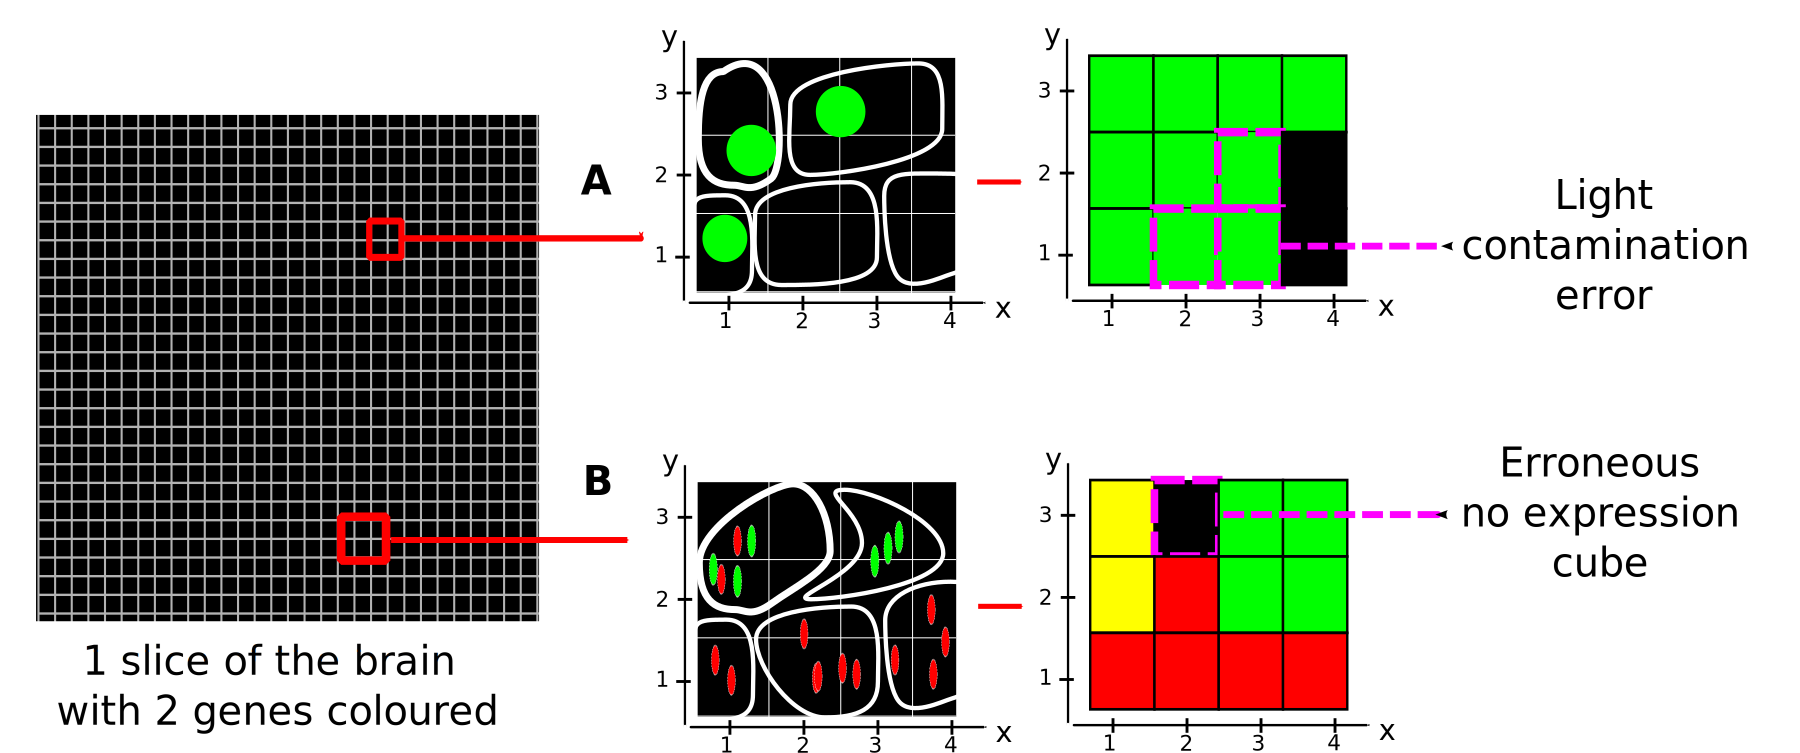
\includegraphics[width=1.3\linewidth]{gfx/chapter2/cubeserrors.png}}
\caption{Errors introduced by the ``cube'' cell model. Path A shows how regions with highly expressed genes can introduce errors through light contamination. Path B shows how some cubes may appear artificially void of expression because of the uneven distribution of transcripts inside the cytoplasm especially for large cells.}\label{fig:cubeserrors}
	\end{figure}
	
	However, even with this simple cell model, the data generated by \citep{Tomer10} is highly valuable. Indeed, not only does this dataset give a snapshot of gene expression for 169 genes in the full brain of \platy{}, it also attaches spatial information to each data point.\\


\section{About the quantitative trait of single cell expression data}\label{sec:quantitative_single_cell}
  \subsection{Light contamination in in-situ hybridization data}
  The light intensity value obtained from in-situ hybridization assays can be considered as a quantitative measure of gene expression \citep{dorresteijn90}. Indeed, the light emitted by every cell in the considered tissue is correlated with the number of RNA fragments of the gene of interest present in the cell as each fragment bound to a probe is an independent source of emission and the probes are hybridized in the cells in large excess. This means that if the targeted gene is highly expressed in a cell, there will be more sources of emission, thus making the overall light intensity captured on this area higher than in a cell expressing the gene at a low level. \\
  
  As mentioned in Section \ref{sec:single_cell_insitu}, in-situ hybridization assays at the single cell level are prone to localized errors due to the cell model. One explanation for those errors, as shown in Figure \ref{fig:cubeserrors}B is the phenomenon of light contamination. When a large group of neighbouring cells express the same gene, the additivity of light intensity mentioned above means that even though the cells express the gene at the same rate, cells surrounded by a lot of other cells expressing the same gene will have abnormally high light intensity readings due to light contamination from the adjacent areas. As a result, when considering a hypothetical circular portion of tissue where a gene is monotonously expressed, the recorded light intensity will show a gradient with the maximum localized on the circle's centre.\\
  
   \begin{figure}[H]
\centerline{\includegraphics[width=0.8\linewidth]{gfx/chapter2/whybina.png}}
\caption{{\bf Light contamination in in-situ hybridization luminescence data seen with the example of the gene Ascl.} Panel A shows the raw fluorescent microscopy capture of the gene's expression for one layer in the brain of Platynereis. Panel B shows the light intensity measured along the red line in panel A. Because of the small scale of study, cells surrounded by other cells expressing a particular gene will have higher intensity values because of nearby light contamination.}\label{fig:why_binarize}
	\end{figure}
  
  As shown in Figure \ref{fig:why_binarize}, the issue of light contamination seems to occur when using the 3 \microm{3} ``cube'' model. In this context, and because of the single cell scale of this study, considering the in-situ hybridization data as quantitative may introduce significant errors. In order to avoid this light contamination bias a solution is to transform the quantitative data into binary data where, for a given ``cube'', genes are simply expressed or not.
  



	
	
  \subsection{Binarizing in-situ hybridization datasets}
	As shown in Figure \ref{fig:why_binarize} and discussed in the previous section \ref{sec:quantitative_single_cell}, the various problems linked to light contamination can be avoided by transforming the ``quantitative'' fluorescence information into binary data. In other words, if $S$ is the set of all ``cubes'' in the brain, $M$ the set of all the considered genes and $y_{i,m}$ the value retrieved from the in-situ hybridization data for ``cube'' $i \in S$ and gene $m \in M$, then  $y_{i,m} = 1$ if gene $m$ is expressed at site $i$, $y_{i,m} = 0$ otherwise. The binarization process itself is not trivial. Indeed, defining the light intensity threshold above which a gene is considered expressed is a complicated problem, especially for noisy data.\\

	Looking at the density of intensities across all the ``cubes'' for each gene yielded two very different scenarios: some densities were separated into two clear peaks, making the threshold easy to find while others exhibited a single peak making it hard to choose a clear cut value as shown in Figure \ref{fig:densities_bina}. After trying different thresholding methods based on those densities, I found, in collaboration with Kaia Achim and Maria Tosches from the Arendt group in EMBL Heidelberg that none of them resulted in binary expression that was satisfying for many genes when compared with a manual inspection of the in-situ hybridization raw images. Considering that this binarized dataset will be the cornerstone of the work presented in this thesis, it was very important to achieve a high confidence thresholding. Given the small number of genes studied (169), and the collaboration with a team of biologists working specifically on \platyfull{}'s brain, a manual thresholding approach was developed. Indeed, by going through the 169 genes one by one, it was possible to adjust the thresholds manually until the resulting binarized expression pattern corresponded perfectly to 1) the fluorescent stack images from in-situ hybridization data; 2) the biologically known expression patterns in the brain of \platy{} expected by the biologists.\\
	
	\begin{figure}[H]
\centerline{\includegraphics[width=0.8\linewidth]{gfx/chapter2/densities_bina.png}}
\caption{{\bf Densities of log luminescence values for two genes (rOpsin, PRDM8) over the $32,302$ cells.} For {\it{rOpsin}}, the density exhibits two clear peaks making the choice of a binarizing threshold easy. By contrast, for {\it{PRDM8}} there is no such clear threshold, making an automated binarization method hard to implement.}\label{fig:densities_bina}
	\end{figure}
	
	This method resulted in a high confidence binarized dataset for $86$ genes. Several reasons explain why $83$ genes out of the starting $169$ were removed from the dataset. For some of the genes no good threshold could be found, this was due to high noise level in the in-situ hybridization images. Other images suffered from experimental errors that yielded blurred and unexploitable expression patterns. Finally some images were polluted by a well known experimental artefact linked to confocal microscopy imaging as shown in Figure \ref{fig:artefact}.\\
	
\begin{figure}[h]
        \myfloatalign
        \subfloat[Z-stack of gene Smad23 showing an experimental artefact (round very bright spot in the middle).]
        {\label{fig:artefact1}
        \includegraphics[width=.45\linewidth]{gfx/chapter2/smad23.png}} \quad
        \subfloat[Z-stack of gene Syt showing an experimental artefact (round very bright spot in the middle).]
        {\label{fig:artefact2}%
         \includegraphics[width=.45\linewidth]{gfx/chapter2/syt.png}}
        \caption{Confocal microscopy experimental artefact for 2 genes of the original $169$ studied genes.}\label{fig:artefact}
\end{figure}
	
	Although the aforementioned method resulted in a high quality binary dataset, it has been possible only because the number of genes considered was small. This will not be the case when dealing with RNA-seq data.
	



\section{Conclusions}
In this Chapter I have described how the scale of gene expression studies has shifted from the tissue level to the single cell level. For two experimental protocols the generation of such data was presented and I have explained why, at the time of writing, it is still not safe to assume that single cell transcritomics datasets are quantitative. To avoid this problem, turning those datasets into binary gene expression is an attractive solution. However the binarization process is not trivial and I have presented ways to obtain a high confidence dataset.\\

One notable advantage of in-situ hybridization assays is the fact that the spatial information stays attached to each gene expression fingerprint. Using this information, it was possible to allocate cells assayed via single cell RNA-seq to their spatial location in the brain using the most specifically expressed genes in every cell. \\

As mentioned previously in the Introduction (\ref{ch:background}), if the ability to study the heterogeneity of cell populations at the single cell level offers incredible possibilities for the future of developmental biology and potentially of cancer research, the development of new statistical methods adapted to this single cell scale, allowing conclusions to be drawn at the tissue level, is crucial.\\

The work presented hereafter aims to answer simple but important questions: can known functional tissues of a complex organ like the brain be defined and localized from single gene expression data? Can unknown regions in such a complex tissue be detected and finally, is it possible to hypothesize the functional role of those unknown regions based on single cell expression data?


	
	



%*****************************************
%*****************************************
%*****************************************
%*****************************************
%*****************************************